\documentclass[compress,handout,10pt]{beamer}

\newlength{\wideitemsep}
\setlength{\wideitemsep}{\itemsep}
\addtolength{\wideitemsep}{100pt}
\let\olditem\item
\renewcommand{\item}{\setlength{\itemsep}{0.5\baselineskip}\olditem}

\usetheme{Singapore}
\usecolortheme{lily}
\usefonttheme[onlymath]{serif}

\usepackage{float}
\floatstyle{boxed}
\usepackage{colortbl}
\usepackage{mathpazo}
\usepackage{graphicx}
\usepackage{movie15}
\usepackage{bm}
\usepackage{verbatim}
\usepackage{comment}
\usepackage{caption}
\usepackage{subcaption}
\captionsetup[subfigure]{labelformat=empty}
\captionsetup[figure]{labelformat=empty}

\newcommand{\mygreen}{\color{green!50!black}}
\newcommand{\myblue}{\color{blue}}
\newcommand{\myred}{\color{red}}
\newcommand{\mycolor}{\color{red}{c}\color{blue}{o}\color{green}{l}\color{orange}{o}\color{cyan}{r}}
\newcommand{\mysize}{\scriptsize{s}\small{i}\normalsize{z}\Large{e}}
\newcommand{\myshape}{\textcircled{s}\textit{h}\texttt{a}\textsf{p}\textsc{e}}

\xdefinecolor{titlecolor}{rgb}{.855,.647,.125}
\setbeamercolor{frametitle}{fg=titlecolor}
\setbeamerfont{frametitle}{series=\bfseries}
\setbeamercolor{normal text in math text}{parent=math text}

\setbeamertemplate{navigation symbols}{} %gets rid of navigation symbols
\setbeamertemplate{footline}[frame number]
\beamertemplateshadingbackground{blue!5}{yellow!10}

\title{{\color{blue} \LARGE  Injury Time in Soccer Game\newline} }

\subtitle{{\color{red} \large Sponsor: FIFA} }

\author{ 
%    \vspace{5pt}
    {\bf{Speaker:}} \\ 
Zhendan Zhu \\ 
    \vspace{5pt}
} 
\institute{JHU AMS 2012 FALL}

\date{\mygreen Last Complied on \today} 

\begin{document}

\begin{frame}[plain]
    \titlepage
\end{frame}

\begin{frame}
    \frametitle{Outline}
    \tableofcontents
\end{frame}

\section{Background}

\begin{frame}
    \frametitle{Background}
    Our project is based on the following background:
    \vspace{7pt}
             \begin{enumerate}
                 \item Rule of Soccer
                 \item Injury time and soccer rule
                 \item Fairness
                 \item FIFA
             \end{enumerate}
\end{frame}


\section{Problem Statement}

\begin{frame}
    \frametitle{Problem Statement}
     \begin{figure}[h]
       \begin{center}
        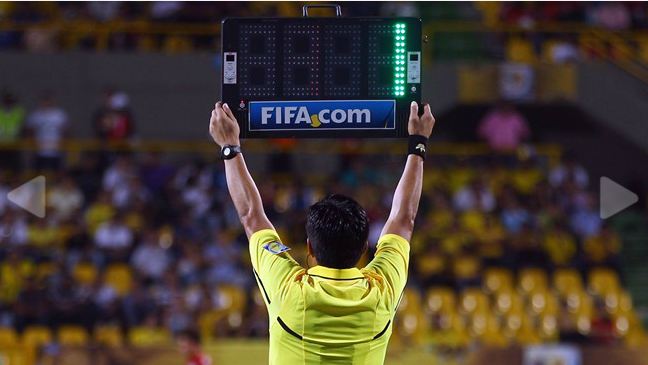
\includegraphics[scale=0.4]{injurytime.png}
    \end{center}
    \caption{The extra minutes may change the score}
    \label{fig:branch}
\end{figure}
\end{frame}

\begin{frame}
    \frametitle{Problem Statement}
     \begin{enumerate}
         \item Two teams, A: distanvantage in 90 mins, B: advantage in 90 mins.
         \item  The referee has the right decide how many minutes to add in injury time.  If the injury time is long enough, A have the chance to catch up and make a tie.
         \item Our problem is to explore the relationship between the length of injury time and the chance of the loser in 90 mins win the game in the end.
         \item Significance of the project
     \end{enumerate}
\end{frame}

\section{Approach}
\begin{frame}
    \frametitle{Approach}
       \begin{enumerate}
         \item  Simplify the problem by a simulation approach based on actual statistics from real games 
     \end{enumerate}
\end{frame}

\begin{frame}
    \frametitle{Approach}
       \begin{enumerate}
         \item  Simplify the problem by a simulation approach based on actual statistics from real games
         \item  Find a distribution for the length between two goals in football game
     \end{enumerate}
\end{frame}

\begin{frame}
    \frametitle{Approach} 
       \begin{enumerate}
         \item  Simplify the problem by a simulation approach based on actual statistics from real games
\cite{IMM1978}
         \item  Find a distribution for the length between two goals in football game
         \item  Collect data from FIFA database, and calcualte the coefficients for the distribution
     \end{enumerate}
\end{frame}

\begin{frame}
    \frametitle{Approach}
       \begin{enumerate}
         \item  Simplify the problem by a simulation approach based on actual statistics from real games
         \item  Find a distribution for the length between two goals in football game
         \item  Collect data from FIFA database, and calcualte the coefficients for the distribution
         \item  Derive a stochastic process for football match, and simulate the results
     \end{enumerate}
\end{frame}

\begin{frame}
    \frametitle{Approach}
       \begin{enumerate}
         \item  Simplify the problem by a simulation approach based on actual statistics from real games
         \item  Find a distribution for the length between two goals in football game
         \item  Collect data from FIFA database, and calcualte the coefficients for the distribution
         \item  Derive a stochastic process for football match, and simulate the results
          \item  Backtesting the simulation results with historical data
     \end{enumerate}
\end{frame}

\section{Milestones}

\begin{frame}
    \frametitle{Milestones}
      \begin{enumerate}
        \item Work Statement due date, Oct 1, 2012,
        \item Midterm Presentation due date, Oct 12, 2012,
        \item Progress Report due date, Oct 26, 2012,
        \item Final Presentation due date, Nov 6, 2012,
        \item Final Report due date, Nov 30, 2012.
     \end{enumerate}
\end{frame}

\section{Deliverable}
\begin{frame}
    \frametitle{From Team to Sponsor}
       \begin{enumerate}
         \item Estiblished model for injury time and game result,
         \item Algorithms for simulating a football game,
         \item Numerical experiment results reporting the effect of injury time to game result,
         \item R package with a complete set of documentations along with some test 
        codes that can be used to reproduce our numerical and simulation test results,
         \item Technical report and presentations summarizing the work. 
         \item  The due date for the project will be Dec.15th
       \end{enumerate}
\end{frame}

\begin{frame}
    \frametitle{From Sponsor to Team}
   \begin{enumerate}
         \item The videos for the matches of major leagues in the world before Oct. 16 2012,
         \item Historical data for each games in five primier leagues and A-level international games,
        \item Symposium attendance travel expenses.
         \item  We need them before Oct.25th
       \end{enumerate}
\end{frame}


\begin{frame}
\bibliographystyle{plain}
\bibliography{biblioMP}
\end{frame}

\end{document}